To evaluate the accuracy of the \osprey \ks algorithm, we performed a series of designs for a variety of protein-protein interfaces (PPIs) as retrospective validation. We used \ks to computationally predict experimentally measured changes in binding for each PPI. Each protein structure is listed by PDB ID in Table \ref{table:spearman} (find more detailed PPI information in Supplemental Table X \anna{this would be where all the systems are listed and potentially all of the mutations we tested}).

\anna{Move to supplemental? "These systems include barnase with its peptide inhibitor barstar, the cytochrome {\it c}/cytochrome {\it c} peroxidase complex, interferon (IFN)$\alpha$2 with its receptor, ifnar2, the interleukin 2 (IL-2)/IL-2 receptor $\alpha$ (IL-2R$\alpha$) complex, and an antibody fragment bound to the I-domain of the integrin VLA1."}

Our retrospective validation experiments focused on mutations at residues in or proximal to the protein-protein interface. Including all such experimentally tested and reported mutations, each structure included anywhere from 5 to 36 ranked designs. Each design included one or two mutable residues along with a set of surrounding flexible residues. Flexible residues were chosen by selecting all residues within 4 \AA of the mutable residues and removing those which only have backbone interactions. 

For each system, the \ks scores were ranked in increasing order of reported experimental binding. Spearman's $\rho$ values were subsequently calculated for each system by calculating the statistical dependence between the \ks score rankings and the experimentally measured rankings. 

\begin{table}[h!]\label{table:spearman}
\centering
\begin{tabular}{ |c||c|  }
 \hline
 \textbf{Structures (PDB ID)}& \textbf{Spearman's $\rho$} \\
 \hline 
 3S9D   & 0.795 \\
 \hline
 1X1U   & 0.755 \\
 \hline
 2B5I   & 0.554 \\
 \hline
 2PCB   & 0.500 \\
 \hline
 1MHP   & 0.365 \\
 \hline 
 \textbf{Across Structures} &   \textbf{0.632}  \\
 \hline
\end{tabular}
\caption{Spearman's $\rho$ table. A Spearman's $\rho$ value is calculated for each system and shown here. The "Across Structures" value is calculated by... }
\end{table}

\begin{figure}\label{fig:rankings}
\center
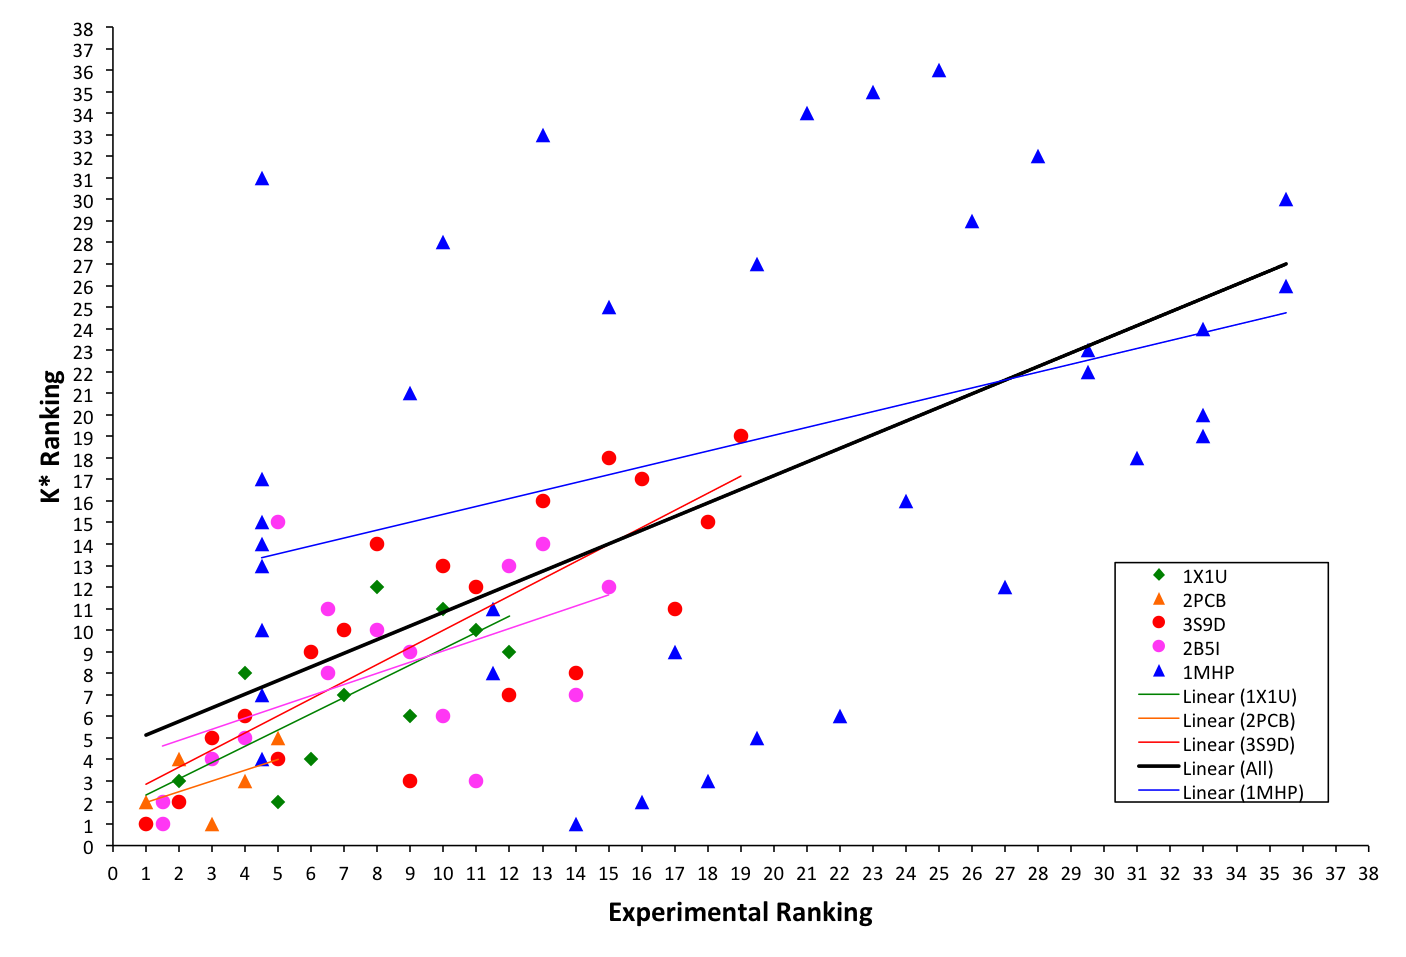
\includegraphics[width=0.9\textwidth]{figures/Rankings.png}
\caption{Testing the accuracy of the \ks algorithm in \osprey3 by comparing \ks rankings to experimentally reported rankings. Each system is represented by its corresponding PDB ID and a linear trendline is shown for each in its corresponding color according to the legend.}
\end{figure}

